
\documentclass[11pt,a4paper,hidelinks,fleqn]{article}            % Article 12pt font for a4 paper while hiding links
\usepackage[margin=1in]{geometry}                          % Required to adjust margins
../styleAndCommands.tex
\date{}
\begin{document}
\subsection*{Question 1 [25 marks]} 
Write a function \verb=MyFirstDeriv(f, x0, h)= to compare three methods of computing the derivative $f'(x_0)$
at point $x_0$ for a function $f(x)$ of an unknown form.
The input \verb=x0= and \verb=h= are two double variables,
and \verb=f= is a function from double to double. 

The first step of \verb=MyFirstDeriv(f, x0, h)= is to construct 5 sample points: $[f(x_0-h), f(x_0-\frac{h}{2}), f(x_0), f(x_0+\frac{h}{2}), f(x_0+h)]$, denoted as \verb=ys=.
Then, it derives the first derivative $f'(x_0)$ in three ways:

\vspace{-6mm}
\paragraph{a)} List the four taylor expansion at the four points $f(x_0-h), f(x_0-\frac{h}{2}), f(x_0+\frac{h}{2}), f(x_0+h)$, 
multiply each by coefficient $b_j$ for $j\in\{1, 2, 3, 4\}$, 
construct a linear system of $b_j$ such that the order 0, 2, and 3 disappear, and order 1 term becomes 1, 
solve for $b_i$, 
print out $b_i$,
derive the coefficients \verb=cs= such that $f'(x_0)$ = \verb=sum(cs .* ys)=,
and print out \verb=cs= and $f'(x_0)$. 
\vspace{-6mm}
\paragraph{b)} Compute $f'(x_0)$ using Richardson extrapolation with the central difference g(h) and the step sizes $h$ and $\displaystyle \frac{h}{2}$,
derived the coefficients \verb=cs= such that $f'(x_0)$ = \verb=sum(cs .* ys)=,
print out \verb=cs= and $f'(x_0)$. Compare the coefficients \verb=cs= with the coefficients derived in part \textbf{a)}.
\vspace{-6mm}
\paragraph{c)} Construct a $4^{th}$ order polynomial $p(x) = \sum_{i=0}^4 a_i x^i$ that passes through the five given points, 
compute $p'(x_0)$ analytically, 
print out the polynomial,
print out the coefficients \verb=cs= such that $p'(x_0)$ = \verb=sum(cs .* ys)=,
and print out the derivative $p'(x_0)$.
Again, compare the coefficients \verb=cs= with the coefficients derived from in \textbf{a)}.


\subsection*{Question 2 [15 marks]}
Numerical minimization of the function
\begin{align*}
f(x) = x^4 - 20 x^2 + 1
\end{align*}
can be viewed as finding roots of the first derivative of f(x),

a) Describe an algorithm for doing this using the secant method.

b) Calculate the first two steps of the algorithm.


\subsection*{Question 3 [20 marks]}
Consider the following one step binomial tree model of the stock price process:
\begin{figure*}[h]
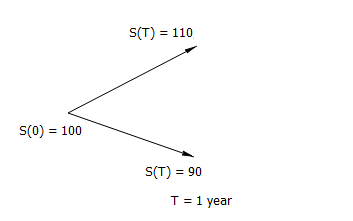
\includegraphics[scale=0.9]{./4}
\end{figure*}

a) Assume interest rate is $0\%$, compute the price of a call option struck at 100 at maturity 1 year?

a) Assume interest rate is $5\%$, compute the price of a call option struck at 100 at maturity 1 year?


\subsection*{Question 4 [20 marks]} 



\subsection*{Question 5 [20 marks]}
Consider the process of a underlying asset $X_t$
\begin{align*}
dX_t = \sigma dW_t
\end{align*}
where $W_t$ is a standard Wiener process and $\sigma$ is the constant volatility.
Denote $V_t$ the price of a derivative on $X_t$. 

a) Derive the partial differential equation satisfied by $V(x, t)$.

b) Discretize the partial differential equation using explicit Euler scheme,
write down the equation that computes $V(x, t_i)$ from the time slice $t_{i+1}$.

c) Suppose that the derivative's price at $t_{i+1}$ is of the following form,
sketch the rough shape of $V(x, t_{i+1})$ on top of the given plot and explain the rationale.
\begin{figure*}[h]
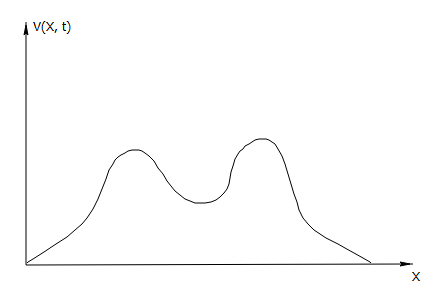
\includegraphics[scale=0.9]{./6c}
\end{figure*}

\textbf{*END OF PAPER*}
\end{document}
